

\newpage
\begin{center}
	\textbf{\large ГЛАВА 1 \\ ПОСТАНОВКА ЗАДАЧИ И ПЛАН РЕШЕНИЯ}
\end{center}
\refstepcounter{chapter}


% \section*{}
\addcontentsline{toc}{chapter}{ГЛАВА 1}
\section{Задачи работы}\label{C1_1}

Создание функционирующего прототипа шагающего робота, приближенного к промышленным моделям, является существенно сложным и дорогостоящим процессом. В связи с этим, для достижения поставленных целей, в данной работе будут применены упрощения, которые окажут влияние на некоторые технические аспекты, однако не повлекут за собой потерю общей ценности исследования - разработки действующего прототипа с готовым управлением, полученным путем решения задач механики и управления без использования методов искусственного интеллекта.


%Задача создания работоспособного прототипа шагающего робота близкого к промышленным образцам является очень сложной и одновременно дорогостоящей работой. По этой причине в рамках работы будут использоваться упрощения, которые повлияют на некоторые технические особенности, но не изменят общей ценности работы – разработки работоспособного прототипа с готовым управлением, полученным путем решения задач механики и управления без применения искусственного интеллекта.
 
Для выполнения данной работы потребуется:
\begin{itemize}
	\item Разработать кинематическую схему ноги робота.
	\item Разработать общую кинематическую схему робота.
	\item Решить обратную задачу кинематики для положения ноги.
	\item Решить задачу описания модели походки робота.
	\item Разработать твердотельную модель ног и корпуса робота.
	\item Подобрать необходимые сервоприводы в сочленения ног робота.
	\item Подобрать комплектующие, связанные с реализацией контроля сервоприводами.
	\item Разработать программное обеспечение для дистанционного управления роботом.
\end{itemize}
\section{Исследование особенностей строения робота}\label{C1_2}
Среди всех компонентов робота, ноги являются наиболее важными составляющими. Такие свойства, как вес, размеры и приведение в действие суставов, непосредственно влияют на производительность движения ног и, следовательно, точность позиционирования робота.

У упомянутых ранее моделей роботов схожи комплекции как корпуса, так и ног, даже общие объемы роботов будут схожи. 
Каждая нога состоит из тазобедренного сустава, бедра, коленного сустава, голени и стопы для контакта с землей, то есть все ноги обладают тремя степенями свободы, а принципы расположения двигателей в ногах имеют минимальное расхождение. Это следствие того, что промышленные модели сделаны из металла и действительно требуют расположения тяжелых двигателей как можно ближе к корпусу для большей устойчивости и меньших затрат на управление. 

В рамках данной работы, робот не обладает существенным весом, а также большими размерами корпуса и ног, в следствие чего будут следующие упрощения:
\begin{itemize}
	\item На одну ногу будет две степени свободы, вместо устоявшегося стандарта в виде трех степеней.
	\item Двигатели будут располагаться в области бедра (у корпуса) и колена (в сочленении ног), так как робот обладает небольшой массой и малыми габаритами для классического решения (рисунок \ref{kinematic}).
\end{itemize}


Последующие упрощения могут привести к утрате возможности контролировать отклонения бедра, что в свою очередь подчеркивает необходимость разработки методов компенсации устойчивости при изменениях углов ориентации корпуса в плоскостях крена и тангажа.
\begin{figure}[h]
	\begin{center}
		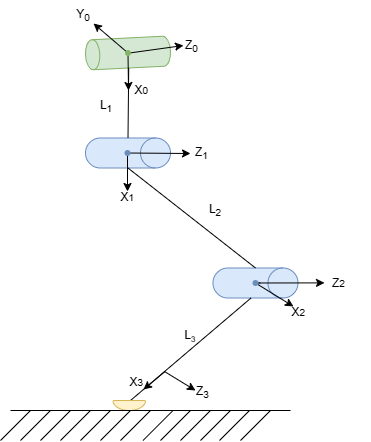
\includegraphics[width=0.3\textwidth]{kinematic}
		\caption{Расположения двигателей для случая 3ех степени свободы на ногу.}
		\label{kinematic}
	\end{center}
\end{figure}


\newpage
